Dalam praktek membuat whatsapp chatbot ini, hal pertama yang harus dilakukan adalah mengenal bahasa pemrograman Python dan mengetahui tentang software yang digunakan yaitu Anaconda3.

\section{Sejarah Python}
Nama python berasal dari acara televisi Monty python's flying circus. Python merupakan bahasa pemrograman yang dikembangkan oleh Guido Van Rossum pada tahun 1990 di CWI, Amsterdam. bahasa ini merupakan lanjutan dari bahasa pemrograman ABC. pada tahun 1995, Guido pindah ke CNRI dan mengeluarkan python versi 1.6. pada tahun 2000, Guido pindah ke BeOpen dan mengeluarkan python versi 2.0 setelah itu Guido dan tim PythonLabs pindah ke  DigitalCreations. saat ini Guido dan Python Software Foundation terus melakukan perkembangan hingga python versi 2.6.1 dan python versi 3.0
Python Software Foundation merupakan sebuah organisasi yang memiliki hak atas bahasa pemrograman python, hal ini dilakukan untuk mencegah bahasa pemrograman python dimiliki oleh perusahaan komersial.

\subsection{Perbedaan Python 2 dan 3}
Perbedaan Python 2 dan Python 3 dapat dilihat pada gambar berikut.
\begin{figure}[!htbp]
        \centerline{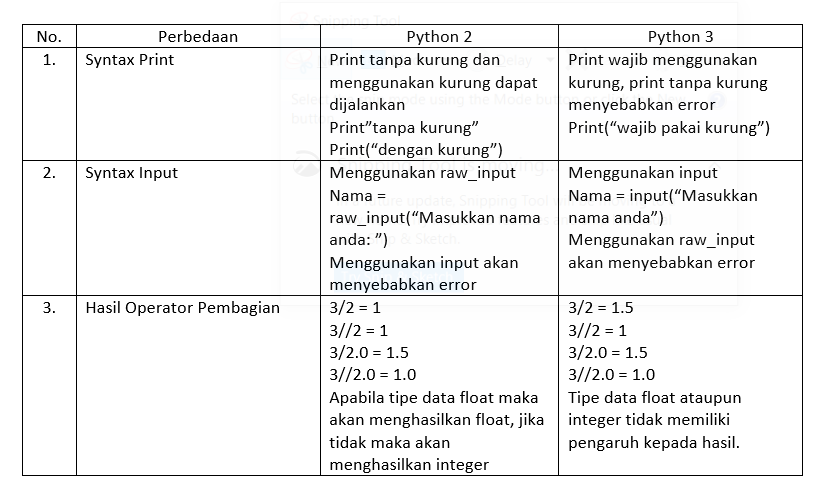
\includegraphics[scale=.75]{figures/perbedaan}}
        \caption{Perbedaan Python 2 dan Python 3}
		\label{perbedaan}
\end{figure}

\subsection{Implementasi dan Penggunaan Python di Perusahaan Dunia}
\begin{enumerate}
\item spotify 
\par
spotify adalah suatu layanan musik streaming yang menggunakan pemrograman python untuk analisis data dan backend. pada backend spotify berkomunikasi dengan 0MQ. 0MQ itu sendiri  adalah suatu framework dan library open source untuk networking. untuk analisis data tersebut spotify menggunakan luigi, dan modul python yang sinkron dengan hadoop.
\item Google
\par 
Google ini sudah menggunakan bahasa pemprograman python ini sudah sajak dari awal berdirinya. Dan pada saat ini bahasa pemprograman python merupakan salah satu bahasa pemprograman server-side resmi di google. Meskipun ada script yang ditulis untuk google menggunakan bahasa perl dan bash, maka nantinya script tersebut akan diubah ke python terlebih dahulu, karena kemudahan dalam perawatannya.
\item Industrial Light and Magic
\par 
Industrial Light and Magic ini merupakan studio special efek yang dibutuhkan untuk film star wars saja. Karena infrastruktur awal industrial light and magisc ini menggunakan C dan C++, maka akan lebih mudah mengintegrasikan bahasa pemprograman python ketimbang bahasa pemprograman lainnya. Dengan menggunakan bahasa pemprogramana python ini industrial light and magic dengan mudah membungkus komponen software dan dapat meningkatkan aplikasi grafisnya.
\item Netflix
\par 
Netflix adalah suatu layanan pemutaran film yang dapat dilakukan oleh pengguna dimanapun dan kapanpun. Pada netfilx bahasa pemprograman yang digunakan adalah bahasa pemprograman python, bahasa pemprograman ini digunakan pada Central Alert Gateway yang akan me-reroute alert dan mengirimkannya pada individu yang akan melihatnya serta juga  dapat secara otomatis reboot atau menghentikan proses yang dianggap bermasalah. Selain itu python juga digunakan untuk menelusuri riwayat dan perubahan pengaturan keamanan.
\item instagram 
\par 
Instagram adalah suatu aplikasi mobile berbasis IOS, android dan windows phone, dimana pengguna dapat berbagi foto dan video melalui instagram ini. Pada instagram ini menggunakan bahasa pemprograman python dalam task queuennya atau fitur dimana setiap pengguna dapat berbagi foto atau video ke beberapa social network lainnya seperti facebook, twitter, dan lain-lainnya.

\end{enumerate}

\subsection{Jenis-Jenis Variabel}
Variabel merupakan tempat penyimpanan data. Tipe data merupakan jenis data yang tersimpan di dalam variabel. terdapat aturan dalam penulisan Variabel.
\begin{enumerate}
 \item Nama variabel diawali dengan huruf atau garis bawah, contoh: nama, \_nama, namaKu, nama\_variabel.
 \item Karakter selanjutnya dapat berupa huruf, garis bawah atau angka, contoh: \_\_nama, nama1, p1.
 \item Karakter bersifat case-sensitive (huruf besar dan huruf kecil dibedakan), contoh: Nama dan NAMA keduanya adalah variabel yang berbeda.
 \item Nama variabel tidak boleh menggunakan kata kunci yang ada pada bahasa pemrograman python, contoh: if, else, while
 \item Nama variabel tidak boleh diawali dengan angka
\end{enumerate}

Jenis-jenis tipe data pada python.
Tipe Data Primitif, dibagi menjadi 3 yaitu:
\begin{enumerate}
 \item Tipe data integer (angka), penulisannya tidak membutuhkan tanda petik, contoh: 10 atau 15
 \item Tipe data string (teks), tipe data string ditandai dengan teks yang diapit oleh tanda petik (""), contoh: "nama saya adalah dinda majesty"
 \item Tipe data boolean (memiliki dua nilai yaitu true dan false atau 0 dan 1)
\end{enumerate}

Contoh penulisan variabel dan tipe datanya:
\begin{enumerate}
 \item angka = 10, angka merupakan nama variabel sedangkan 10 adalah nilai dari variabel yang tipe datanya integer.
 \item nama = "Dinda Majesty", nama merupakan nama variabel sedangkan "Dinda Majesty" merupakan nilai dari variabel yang tipe datanya string, ditandai dengan adanya petik ("").
 \item makan = True , makan merupakan nama variabel sedangkan True merupakan nilai dari variabel yang tipe datanya boolean.
\end{enumerate}

\subsection{Input dan Output}
Berikut kode untuk meminta inputan dari user.
\lstinputlisting[caption=Input dan Output , language=Python, firstline=7, lastline=10]{src/teori.py}
Perintah input() berguna untuk meminta inputan dari user, sehingga memungkinkan user untuk menginputkan data.\\
Perintah print() berguna untuk menampilkan output dari data yang diinputkan oleh user, sehingga data yang diinputkan user dapat ditampilkan ke layar.

\subsection{Operator Aritmatika dan Konversi Tipe Data}
Operator aritmatika
\begin{enumerate}
 \item penjumlahan (+)
 \item pengurangan (-)
 \item perkalian (*)
 \item pembagian (/)
 \item sisa bagi/modulus (%)
 \item pemangkatan (**)
\end{enumerate}
Cara melakukan perubahan terhadap tipe data string menjadi integer, contoh: variabel = "10". Kita dapat mengubah string "10" menjadi angka 10 dengan menambahkan kode int(variabel), dengan begitu 10 yang awalnya bertipe data string akan dikonversikan menjadi integer.\\
Cara melakukan perubahan terhadap tipe data integer menjadi string, contoh: variabel = 150. Kita dapat mengubah integer 150 menjadi string "150" dengan menambahkan kode str(variabel), maka tipe data dari variabel akan dikonversikan menjadi string.

\subsection{Perulangan}
perulangan terdiri atas 3 kondisi.
\begin{enumerate}
 \item While, apabila kondisinya True, maka perulangan akan terus berjalan hingga diperoleh kondisi False. Contoh penggunaan while:\\
\lstinputlisting[caption=While Loop , language=Python, firstline=12, lastline=18]{src/teori.py}
 \item For, perulangan for bisa melakukan perulangan terhadap item apapun seperti list atau string. Contoh penggunaan For:\\
\lstinputlisting[caption=For Loop , language=Python, firstline=20, lastline=23]{src/teori.py}
 \item nested, perulangan ini memungkinkan adanya perulangan didalam perulangan. Contoh penggunaan nested:\\
\lstinputlisting[caption=Nested Loop , language=Python, firstline=25, lastline=35]{src/teori.py}
\end{enumerate}
Pada penulisan sintaks While dan For harus memperhatikan identasi (baris yang menjorok ke dalam), jika tidak diperhatikan dengan baik maka akan terjadi error terhadap identasi. Untuk menambahkan identasi dapat menggunakan spasi atau tab.

\subsection{IF Statement}
kondisi if dapat digunakan didalam looping dan dapat digunakan untuk memberikan kondisi tertentu dengan cara mengetikkan if lalu kondisi yang akan terjadi.\\
\begin{enumerate}
 \item if hanya menjalankan satu kondisi dan menampilkan satu output. Contoh: kondisi dimana variabel a lebih besar dari variabel b, maka tampilkan hasil bahwa a lebih besar dari b.
\lstinputlisting[caption=if Statement , language=Python, firstline=37, lastline=41]{src/teori.py}
 \item elif digunakan apabila kondisi pertama tidak benar maka lakukan kondisi lain (alternatif). Contoh: kondisi dimana variabel a sama dengan variabel b, maka jika b lebih besar dari a, tampiilkan hasil b lebih besar dari a, namun jika a dan b bernilai sama, maka tampilkan a sama dengan b
\lstinputlisting[caption=Elif , language=Python, firstline=43, lastline=49]{src/teori.py}
\item else digunakan apabila kondisi yang terjadi bernilai salah, maka lakukan else. Contoh: kondisi dimana variabel a lebih besar dari variabel b, maka jika b lebih besar dari a, tampiilkan hasil b lebih besar dari a, jika a dan b bernilai sama, maka tampilkan a sama dengan b, jika salah maka tampilkan a lebih besar dari pada b
\lstinputlisting[caption=Else , language=Python, firstline=51, lastline=59]{src/teori.py}
\item Nested if merupakan if didalam if (if bersarang), terdapat dua if didalam satu kondisi. Contoh: variabel x sama dengan 41, kondisi pertama yaitu jika x besar dari 10 maka tampilkan lebih besar dari 10, kondisi kedua yaitu jika x besar dari 20, maka tampilkan lebih besar dari 20, jika salah maka tampilkan tidak melebihi 20.
\lstinputlisting[caption=Nested If , language=Python, firstline=61, lastline=69]{src/teori.py}
\end{enumerate}

\section{Praktek Pertama Python}
\subsection{Modulus}
Praktek kali ini kita akan mencoba praktek menggunakan modulus atau sisa bagi, kita membuat inputan terlebih dahulu menggunakan perintah input. Kemudian buatlah variabel untuk menampung hasil sisa bagi dari jumlah yang diinputkan. Misalnya, teman-teman menginputkan nilai yaitu 1184011, maka hasil modulus 1184011 mod 3 adalah 1 maka print 1184011 menggunakan tanda pagar. jika hasil modulus adalah 0 maka print 1184011 menggunakan tanda bintang.
\lstinputlisting[caption=Modulus, language=Python, firstline=7, lastline=24]{src/1184011.py}
\subsection{Hello NPM}
Setelah selesai praktek modulus kita akan menampilkan output berupa kalimat "Hello 1184011 Apa Kabar" sebanyak 2 digit belakang angka, yaitu angka 11, maka akan berulang sebanyak 11 kali.
\lstinputlisting[caption=Hello NPM, language=Python, firstline=26, lastline=32]{src/1184011.py}
\subsection{Hello NPM (3 Digit Belakang)}
Jika telah selesai, maka selanjutnya kita akan melakukan praktek untuk menampilkan output berupa kalimat "Hallo 011 Apa Kabar?" sebanyak angka keenam ditambah angka ketujuh atau 1 ditambah 1, sehingga kalimat tersebut akan berulang sebanyak 2 kali.
\lstinputlisting[caption=3 Digit Belakang, language=Python, firstline=34, lastline=42]{src/1184011.py}
\subsection{Hello NPM (Digit ke-3)}
Kemudian kita akan melakukan praktek untuk menampilkan output berupa kalimat "Hallo 0 Apa Kabar?".
\lstinputlisting[caption=Digit ke-3, language=Python, firstline=44, lastline=48]{src/1184011.py}
\subsection{Variabel Alfabet}
Teman-teman, sekarang mari kita coba menambahkan variabel pada angka 1184011, tambahkan abcdefg kedalam sebuah variabel dan tambahkan variabel index dengan nilai 0, buatlah perulangan agar variabel huruf menyesuaikan dengan variabel angka sehingga menjadi a=1, b=1, c=8, d=4, e=0, f=1 ,g=1.
\lstinputlisting[caption=Variabel Alfabet, language=Python, firstline=50, lastline=58]{src/1184011.py}
\subsection{Penjumlahan NPM}
Praktek selanjutnya adalah menjumlahkan angka 1184011 dengan menerapkan perulangan dan penambahan. Apabila nilai 1 telah didapatkan maka akan ditambahkan dengan nilai 1 sehingga menjadi 2, kemudian nilai 2 ditambahkan lagi dengan nilai selanjutnya yaitu 8 sehingga menjadi 10, begitu seterusnya.
\lstinputlisting[caption=Penjumlahan NPM, language=Python, firstline=60, lastline=71]{src/1184011.py}
\subsection{Perkalian NPM}
Praktek selanjutnya adalah mengalikan angka 1184011 dengan menerapkan perulangan dan perkalian. Apabila nilai 1 telah didapatkan maka akan dikalikan dengan nilai 1 sehingga menjadi 1, kemudian nilai 1 dikalikan lagi dengan nilai selanjutnya yaitu 8 sehingga menjadi 8, begitu seterusnya.
\lstinputlisting[caption=Perkalian NPM, language=Python, firstline=73, lastline=84]{src/1184011.py}
\subsection{Print Vertical}
Melakukan print secara vertikal hanya perlu menambahkan perulangan terhadap nilai 1184011.
\lstinputlisting[caption=Print Vertical, language=Python, firstline=86, lastline=90]{src/1184011.py}
\subsection{Digit Genap NPM}
Selanjutnya, mari kita lakukan print hanya terhadap digit genap pada angka 1184011 dengan memanfaatkan perulangan, if statement dan operator logika. Logika yang akan diterapkan adalah masing-masing angka 1184011 akan di cek terlebih dahulu, apakah angka tersebut memiliki angka yang apabila dibagi 2 akan menghasilkan sisa bagi sama dengan 0 dan angka tersebut tidak boleh sama dengan 0, karena angka 0 bukan merupakan angka ganjil maupun genap.
\lstinputlisting[caption=Digit Genap NPM, language=Python, firstline=92, lastline=99]{src/1184011.py}
\subsection{Digit Ganjil NPM}
Selanjutnya, mari kita lakukan print hanya terhadap digit ganjil pada angka 1184011 dengan memanfaatkan perulangan, if statement dan operator logika. Logika yang akan diterapkan adalah masing-masing angka 1184011 akan di cek terlebih dahulu, apakah angka tersebut memiliki angka yang apabila dibagi 2 akan menghasilkan sisa bagi tidak sama dengan 0 dan angka tersebut tidak boleh sama dengan 0, karena angka 0 bukan merupakan angka ganjil maupun genap.
\lstinputlisting[caption=Digit Ganjil NPM, language=Python, firstline=101, lastline=108]{src/1184011.py}
\subsection{Bilangan Prima NPM}
Praktek terakhir adalah menampilkan hasil dari bilangan prima angka 1184011 dengan cara apabila angka 1184011 memiliki angka yang merupakan angka prima maka akan ditampilkan, logika yang akan diterapkan adalah apabila angka kecil sama dengan angka 1 maka angka tersebut bukan bilangan prima. Jika angka 1184011 dibagi 2 setelah itu dibagi dengan angka itu sendiri dan menghasilkan sisa bagi sama dengan 0, maka angka tersebut bukan bilangan prima
\lstinputlisting[caption=Bilangan Prima NPM , language=Python, firstline=110, lastline=126]{src/1184011.py}

\section{Peringatan Error dan Cara Mengatasinya}
\begin{enumerate}
 \item NameError, terjadi apabila kode mengeksekusi nama yang tidak terdefenisikan. Contoh:
 \begin{verbatim}
 nama = "Dinda Majesty"
 print(Nama)
 \end{verbatim}
 Maka akan menghasilkan output NameError: name 'Nama' is not defined. error ini dapat diatasi dengan mengubah variabel yang di print sesuai dengan variabel yang didefenisikan, karena penulisan pada pyton bersifat case-sensitive
 
 \item SyntaxError, terjadi apabila kode python mengalami kesalahan saat penulisan. Contoh: menuliskan variabel yang didahului angka (1nama = "Dinda Majesty") maka akan muncul eror SyntaxError: invalid syntax. error ini dapat diatasi dengan memperhatikan tata cara penulisan kode pada bahasa pemrograman python.
 
 \item TypeError, terjadi apabila kode melakukan operasi atau fungsi terhadap tipe data yang tidak sesuai. Contoh: melakukan penjumlahan terhadap tipe data string dan integer. eror ini dapat diatasi dengan mengubah tipe data string menjadi integer.
 \begin{verbatim}
 a = "10"
 b = 5

 print(a + b)
 \end{verbatim}
 Maka akan menghasilkan output eror TypeError: can only concatenate str (not "int") to str
 
 \item IdentationError, terjadi apabila kode perulangan atau pengkondisian tidak menjorok kedalam (tidak menggunakan identasi), error ini dapat diatasi dengan menambahkan tab atau spasi. Contoh:
 \begin{verbatim}
 a = 200
 b = 330
 if b > a:
 print("b lebih besar dari a")
 \end{verbatim}
 Maka akan menghasilkan output eror IndentationError: expected an indented block
\end{enumerate}

\subsection{Except}
Try Except merupakan perintah yang bisa digunakan dalam penanganan error pada bahasa pemrograman python. perintah ini biasanya digunakan saat penanganan error input/output, operasi database, pengaksesan indeks suatu list atau dictionary dan berbagai kasus lainnya.\\
Contoh sederhana penggunaan Try-Except saat menangani NameError
\lstinputlisting[caption=Try Except , language=Python, firstline=71, lastline=77]{src/teori.py}
Pada contoh diatas, try except akan menghasilkan output Variabel x tidak ada, karena kita tidak mendefinisikan variabel x sebelum kita menampilkan output x ke layar. Dengan menggunakan try except kode yang kita buat terhindar dari error dan kita bisa mengetahui kesalahan yang terjadi ketika terdapat error pada kode kita.

\subsection{Run Script Hello World di Spyder}
Jika teman-teman telah berhasil melakukan instalasi anaconda3 maka teman-teman akan memiliki sofware spyder, pada software ini teman-teman akan mengetikkan kode program yang akan teman-teman buat nantinya. Sekarang ayo kita coba menjalankan program untuk mencetak kata \textit{hello world}.
\begin{enumerate}
\item Buka anaconda navigator, lalu klik launch seperti pada gambar \ref{Anaconda Navigator}.
\begin{figure}[!htbp]
    \centering
    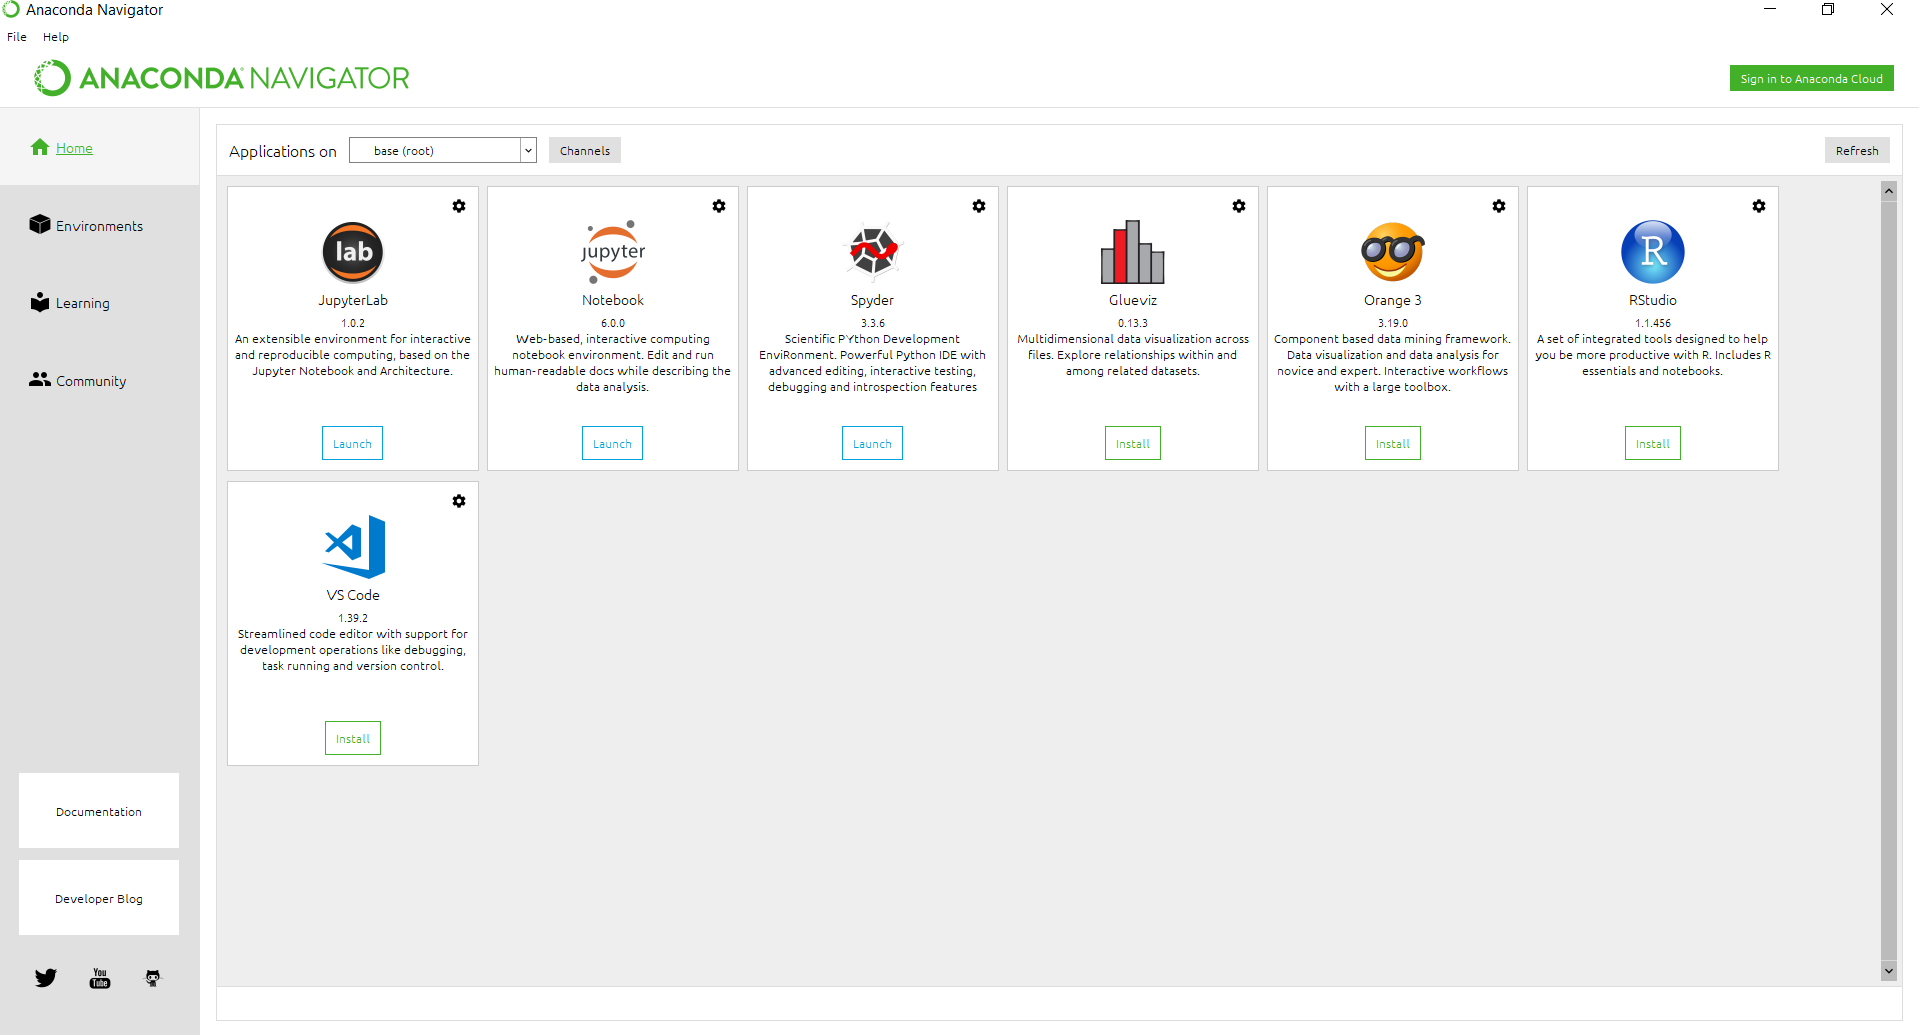
\includegraphics[scale=0.3]{figures/navigator}
    \caption{\textit{Launch Spider}}
    \label{Anaconda Navigator}
\end{figure}
\item ketikkan print("Hello World") dan run spyder dengan cara mengklik tombol berwarna hijau yang terletak ditengah toolbar, untuk lebih jelas dapat dilihat pada gambar \ref{Print Hello World}.
\begin{figure}[!htbp]
    \centering
    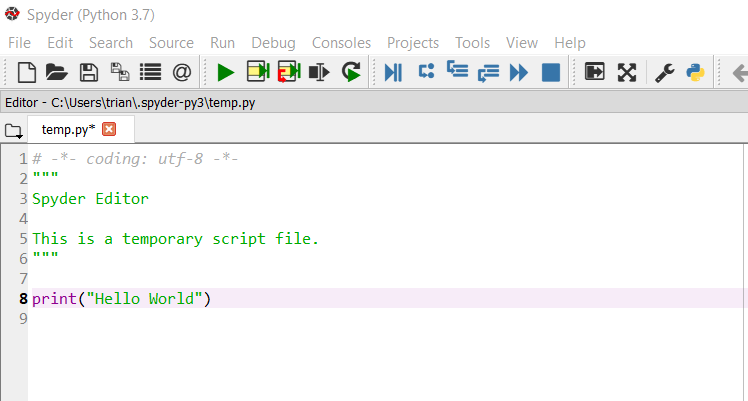
\includegraphics[scale=0.75]{figures/helloworld}
    \caption{\textit{Print Hello World}}
    \label{Print Hello World}
\end{figure}
\item hasilnya akan tampak seperti pada gambar \ref{Hello World}
\begin{figure}[!htbp]
    \centering
    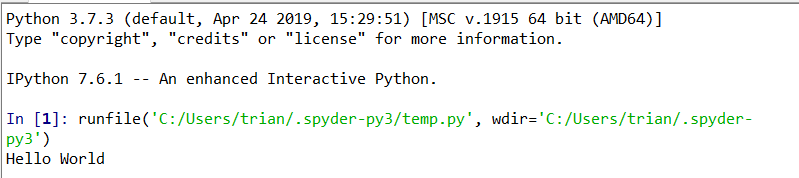
\includegraphics[scale=0.75]{figures/run}
    \caption{\textit{Hello World}}
    \label{Hello World}
\end{figure}
\end{enumerate}

\subsection{Pemakaian Variable Explorer}
Variable explorer akan secara otomatis terisi ketika kita membuat variable, pada variable explorer kita bisa melihat nama variable, tipe data, length, dan value dari variable tersebut. Contoh penggunaan variabel explorer dapat teman-teman lihat pada gambar \ref{Variable Explorer}.
\begin{figure}[!htbp]
    \centering
    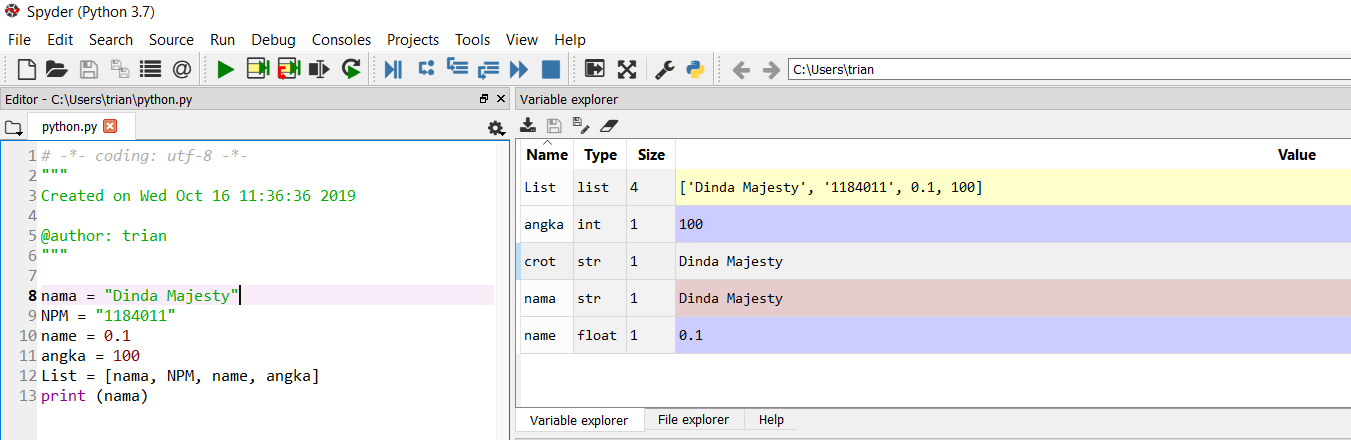
\includegraphics[scale=0.4]{figures/variable}
    \caption{\textit{Variable Explorer}}
    \label{Variable Explorer}
\end{figure}

\section{Indentasi}
\subsection{Penjelasan Indentasi}
Identasi adalah bagian paragraf yang menjorok ke dalam pada baris-baris paragraf. Mengatur indentasi dapat menggunakan tab atau spasi. Identasi digunakan oleh bahasa pemrograman python sebagai pengganti briket ({}) untuk membuka dan menutup fungsi. Error indentasi dapat terjadi apabila syntax tidak menggunakan tab atau space.
Contoh yang benar (menggunakan tab/spasi sebagai indentasi):
\begin{verbatim}
# blok percabangan if
if username == 'petanikode':
    print("Selamat Datang Admin")
    print("Silahkan ambil tempat duduk")

# blok percabangan for
for i in range(10):
    print i
\end{verbatim}
Contoh yang salah (tidak menggunakan tab/spasi):
\begin{verbatim}
# blok percabangan if
if username == 'petanikode':
print("Selamat Datang Admin")
print("Silahkan ambil tempat duduk")

# blok percabangan for
for i in range(10):
print i
\end{verbatim}

\subsection{Jenis-Jenis Error Indentasi}
IndentationError: unexpected indent. Error diatas terjadi apabila syntax kekurangan tab atau spasi. Contoh error identasi dapat dilihat pada gambar \ref{Indentasi}.
\begin{figure}[!htbp]
    \centering
    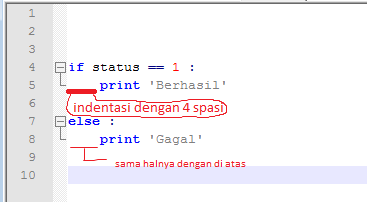
\includegraphics[scale=0.6]{figures/indentasi}
    \caption{\textit{Indentasi}}
    \label{Indentasi}
\end{figure}
Apabila di running akan memunculkan error seperti pada gambar \ref{Error Indentasi}.
\begin{figure}[!htbp]
    \centering
    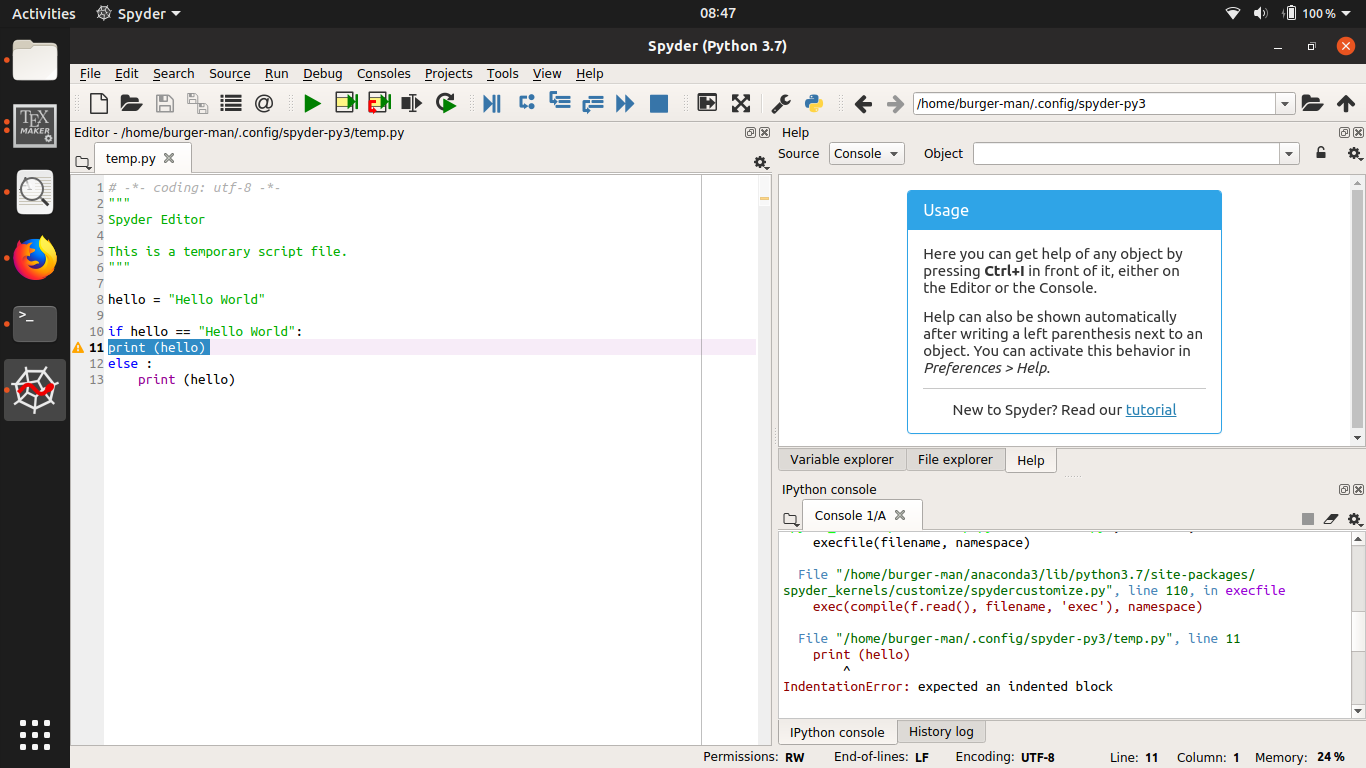
\includegraphics[scale=0.6]{figures/errorindentasi}
    \caption{\textit{Error Indentasi}}
    \label{Error Indentasi}
\end{figure}

\subsection{Cara Membaca Error}
Jika terjadi error maka cari di line berapa error terjadi, pada gambar \ref{Error Indentasi} terdapat error indentasi pada line 10.


\subsection{Cara Menangani Error}
Menangani error indentasi dapat dilakukan dengan cara menambahkan tab atau space pada line yang error. Untuk lebih jelasnya dapat teman-teman lihat pada gambar \ref{Syntax Error}.
\begin{figure}[H]
    \centering
    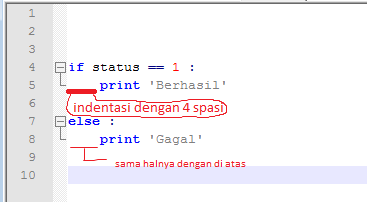
\includegraphics[scale=0.7]{figures/indentasi}
    \caption{\textit{Syntax Error}}
    \label{Syntax Error}
\end{figure}
Penulisan syntax identasi yang benar dapat dilihat pada gambar \ref{Syntax Error1}.
\begin{figure}[H]
    \centering
    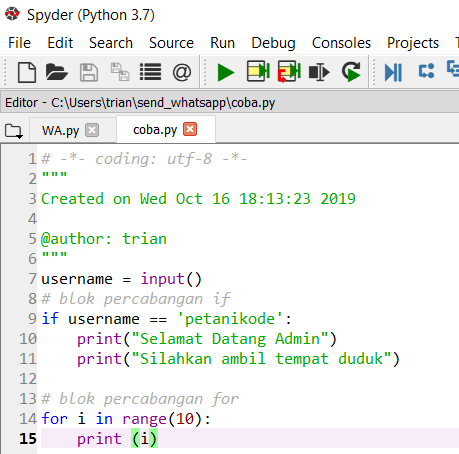
\includegraphics[scale=0.8]{figures/indentasicoy}
    \caption{\textit{Syntax yang Telah Diperbaiki}}
    \label{Syntax Error1}
\end{figure}

\subsection{Quiz: 1}
\begin{enumerate}
\item Siapakah pencipta Python?\\
a) Guido van Rossum\\
b) Guido van Persie\\
c) Guido van Linguini\\
d) Guido van Laptop

\item Pada tahun berapa python dikembangkan?\\
a) 1999\\
b) 1995\\
c) 1945\\
d) 1990

\item Apa itu indentasi?\\
a) Bagian paragraf yang menjorok ke dalam\\
b) Bagian paragraf yang menjorok ke sungai\\
c) Bagian paragraf yang menjorok ke laut\\
d) Bagian paragraf yang menjorok ke hati

\item Apa itu try except?\\
a) Perintah untuk penanganan masalah hidup\\
b) Perintah untuk penanganan masalah error\\
c) Perintah untuk penanganan masalah galau\\
d) Perintah untuk penanganan masalah sakit perut

\item Apa itu if statement?\\
a) Kondisi yang digunakan untuk percabangan logika\\
b) Kondisi yang digunakan untuk percabangan pohon\\
c) Kondisi yang digunakan untuk percabangan tunas\\
d) Kondisi yang digunakan untuk percabangan akar
\end{enumerate}